% BEGIN PREAMBEL
\documentclass[9pt]{beamer}
\usepackage[british]{babel}
\usepackage[latin1]{inputenc}
\usepackage{amsmath,amsfonts,amssymb}
\usepackage{upgreek}
\usepackage{pgfpages}
\usepackage[version=3]{mhchem}
\usepackage{lmodern}
\usepackage{graphicx}
\usepackage{multicol}
\usepackage{xcolor}
\usepackage{wrapfig}
\newcommand{\as}{\\[14pt]}
\newcommand{\s}{\\[7pt]}
\newcommand{\is}{\\[2pt]}
\newcommand{\no}{\noindent}
\newcommand{\ka}{\hspace*{0.5cm}}
\newcommand{\ma}{\hspace*{1cm}}
\newcommand{\ga}{\hspace*{1.5cm}}
\newcommand{\li}{\left|}
\newcommand{\re}{\right|}
\newcommand{\const}{\text{const.}}
\newcommand{\z}{\text}
\newcommand{\terminal}[1]{\colorbox{black}{\textcolor{white}{{\fontfamily{phv}\selectfont \scriptsize{#1}}}}}
\newcommand{\plugin}[1]{\textit{\flq#1\frq}}
\usetheme{Boadilla}
\usecolortheme{beaver}
\useoutertheme{miniframes}
\graphicspath{ {Pics/} }
\beamertemplatenavigationsymbolsempty
\makeindex
\title[ETH High Rate Beam Telescope]{ETH High Rate Beam Telescope}
\author[M. Reichmann]{Michael Reichmann}
\institute[\textbf{\textit{ETH}}\scalebox{.6}{\textit{Z\"{u}rich}}]{Swiss Federal Institute of Technology Zurich}
% END PREAMBEL
\begin{document}
% ============================
% TITLE PAGE
% ============================
\begin{frame}
	\begin{center}
		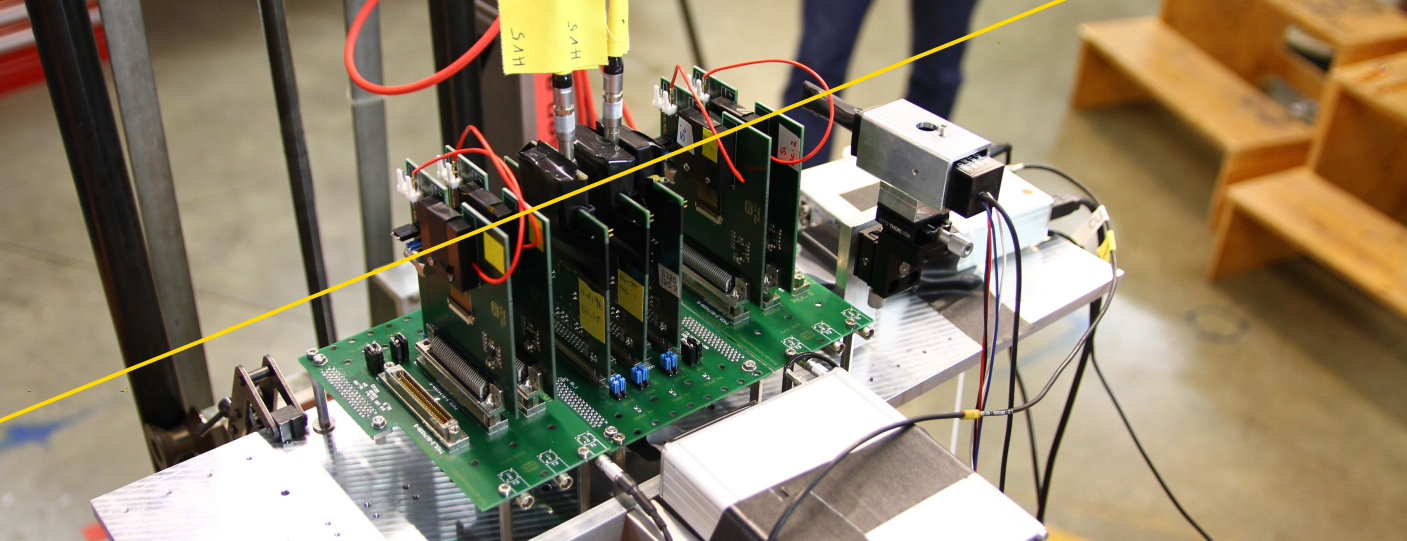
\includegraphics[width=10cm]{Pics/telescope1}
	\end{center}
	\begin{alertblock}{
		\begin{center}
			\textbf{ETH High Rate Beam Telescope}
		\end{center}}
		\vspace*{10pt}
		\begin{center}\small
			presented by: Michael Reichmann \\ 
			coauthors: Felix Bachmair, Dmitry Hits
		\end{center}\normalsize
	\end{alertblock}
\end{frame}
% ============================
% TABLE OF CONTENTS
% ============================
\begin{frame}%[allowframebreaks]
	\frametitle{Table of contents}
	\tableofcontents[hideallsubsections]   % [pausesections]
\end{frame}
% ====================================================================================
% MOTIVATION
% ====================================================================================
\section{Motivation}
\begin{frame}
	\begin{alertblock}{
		\begin{center}
			\Large{\textbf{Motivation}}
		\end{center}}
	\end{alertblock}
\end{frame}
% new frame ============================
\begin{frame}
	\underline{\textbf{Conditions:}}
	\begin{itemize}
		\item testing of diamond pad and pixel detectors for rate dependence
		\item continous pion beam with a flux of up to $100\,\z{MHz/cm}^{2}$ and momenta of $100$-$500$\,MeV
	\end{itemize}
	\underline{\textbf{Requirements:}}
	\begin{itemize}
		\item small, flexible and modular system
		\item high rate continuous data taking
		\item adjustable trigger area to reduce pedestal events
	\end{itemize}
\end{frame}
% ====================================================================================
% TELESCOPE
% ====================================================================================
\section{The Telescope}
\begin{frame}
	\begin{alertblock}{
		\begin{center}
			\Large{\textbf{The Telescope}}
		\end{center}}
	\end{alertblock}
\end{frame}
% ============================
% GENERAL SETUP
\subsection{General Setup}
\begin{frame}
	\frametitle{General Setup}
	\begin{center}
		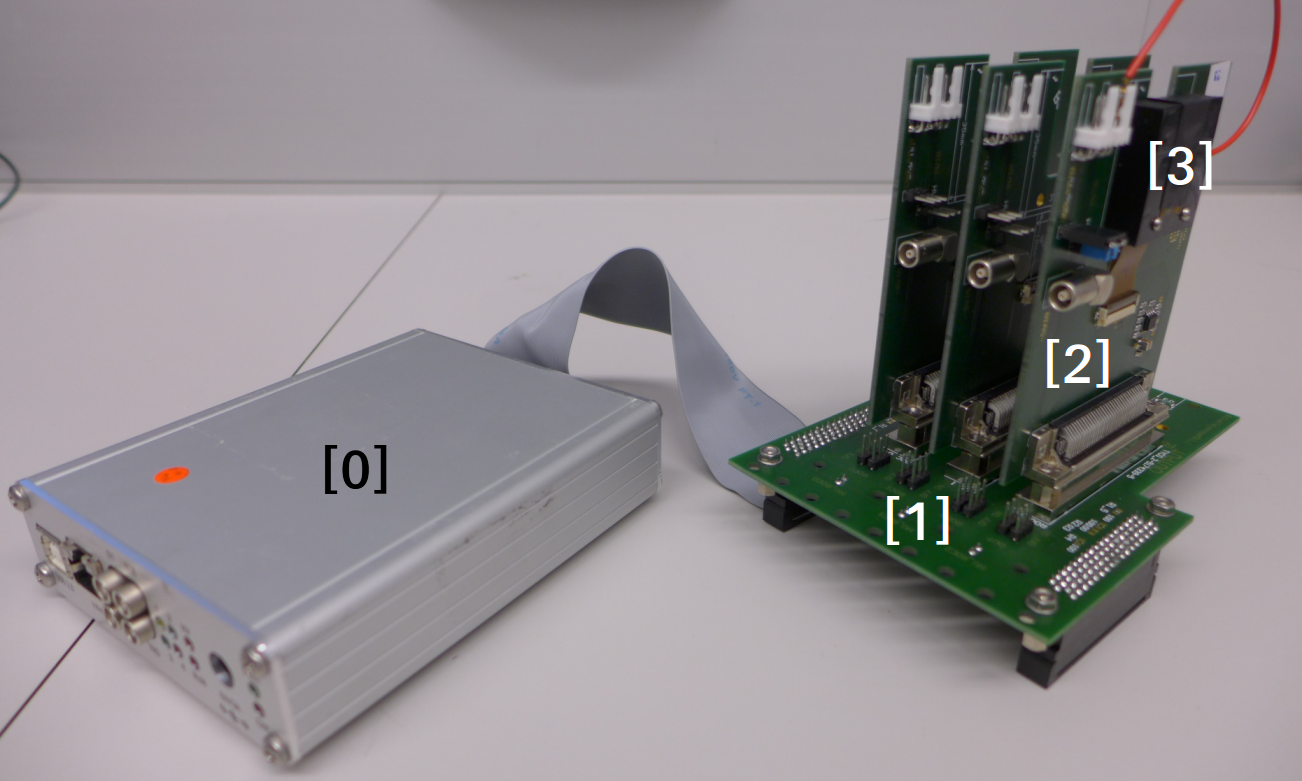
\includegraphics[width=8cm]{Pics/setup}
	\end{center}
	\begin{itemize}
		\item $[0]$ DTB (Digital Test Board): interface to a computer
		\item $[1]$ Motherboard: main frame of the telescope
		\item $[2]$ Adapter Planes: mounting framework for the single pixel chips
		\item $[3]$ CMS Pixel Chip (analogue or digital)
	\end{itemize}
\end{frame}
% ============================
% MOTHERBOARD
\subsection{Motherboard}
\begin{frame}
	\frametitle{Motherboard}
	\begin{center}
		\begin{minipage}{4.6cm}
			\centering
			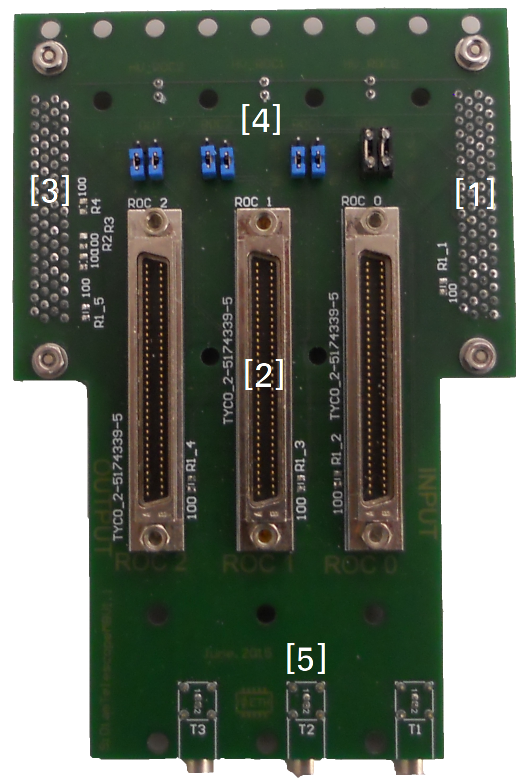
\includegraphics[width=4.5cm]{Pics/Motherboard}
		\end{minipage}
		\hspace*{2pt}
		\begin{minipage}{6cm}
			\begin{itemize}
				\item $[1]$ input: SCSI connector to the DTB
				\item $[2]$ sockets for the adapter planes
				\item $[3]$ output (optional): SCSI connector to another motherboard
				\item $[4]$ token jumpers: (blue = plane active, black = plane inactive) 
				\item $[5]$ output of the fast-OR trigger signal 
				\item $[6]$ termination of the signals
			\end{itemize}
		\end{minipage}\no\s
	\end{center}
\end{frame}
% ============================
% PLANE
\subsection{Adapter Planes}
\begin{frame}
	\frametitle{Adapter Planes}
	\begin{center}
		\begin{minipage}{5.5cm}
			\centering
			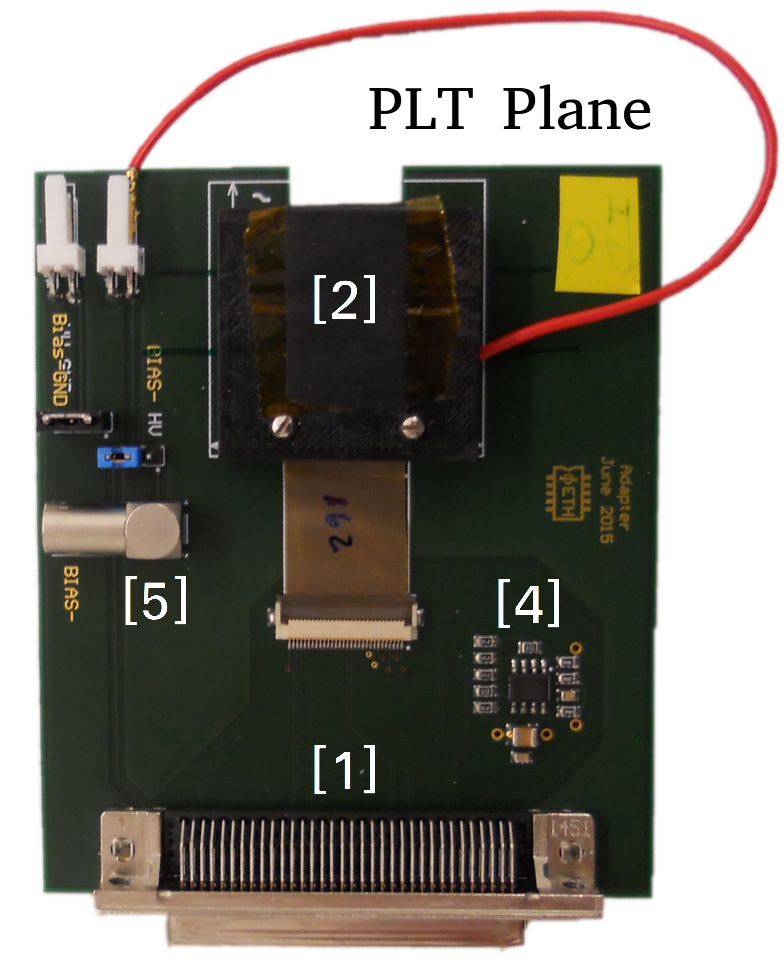
\includegraphics[width=3.4cm]{Pics/AdapterAnalog}
		\end{minipage}
		\hspace*{2pt}
		\begin{minipage}{5.5cm}
			\centering
			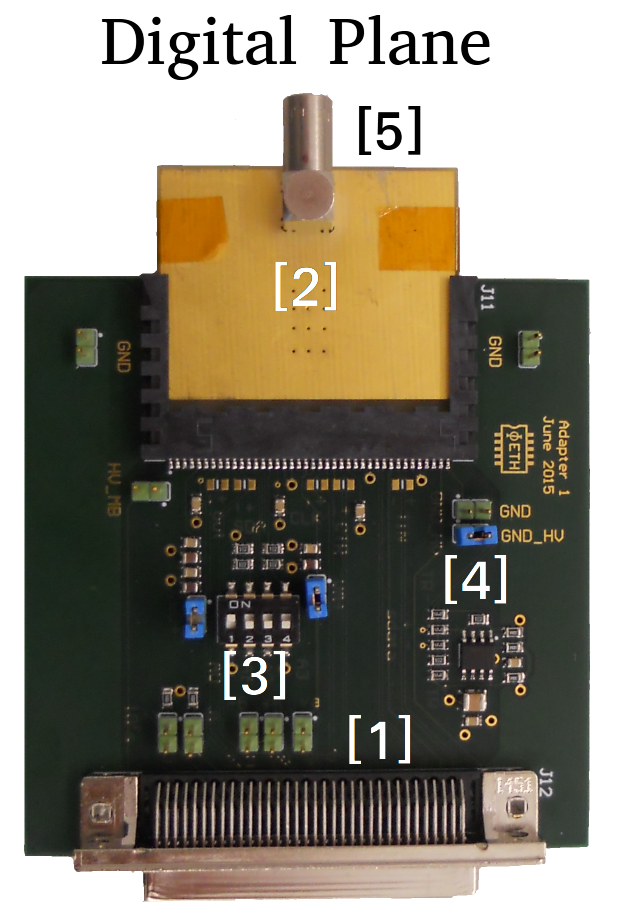
\includegraphics[width=2.8cm]{Pics/AdapterDigital}
		\end{minipage}
	\end{center}
	\begin{itemize}
		\item $[1]$ SCSI connector to MB
		\item $[2]$ CMS pixel chip
		\item $[3]$ bit switch for I$^{2}$C address
		\item $[4]$ amplifying circuit
		\item $[5]$ sensor bias input
	\end{itemize}
\end{frame}
% ============================
% MODULARITY
\subsection{Modularity}
\begin{frame}
	\frametitle{Modularity}
	\begin{center}
		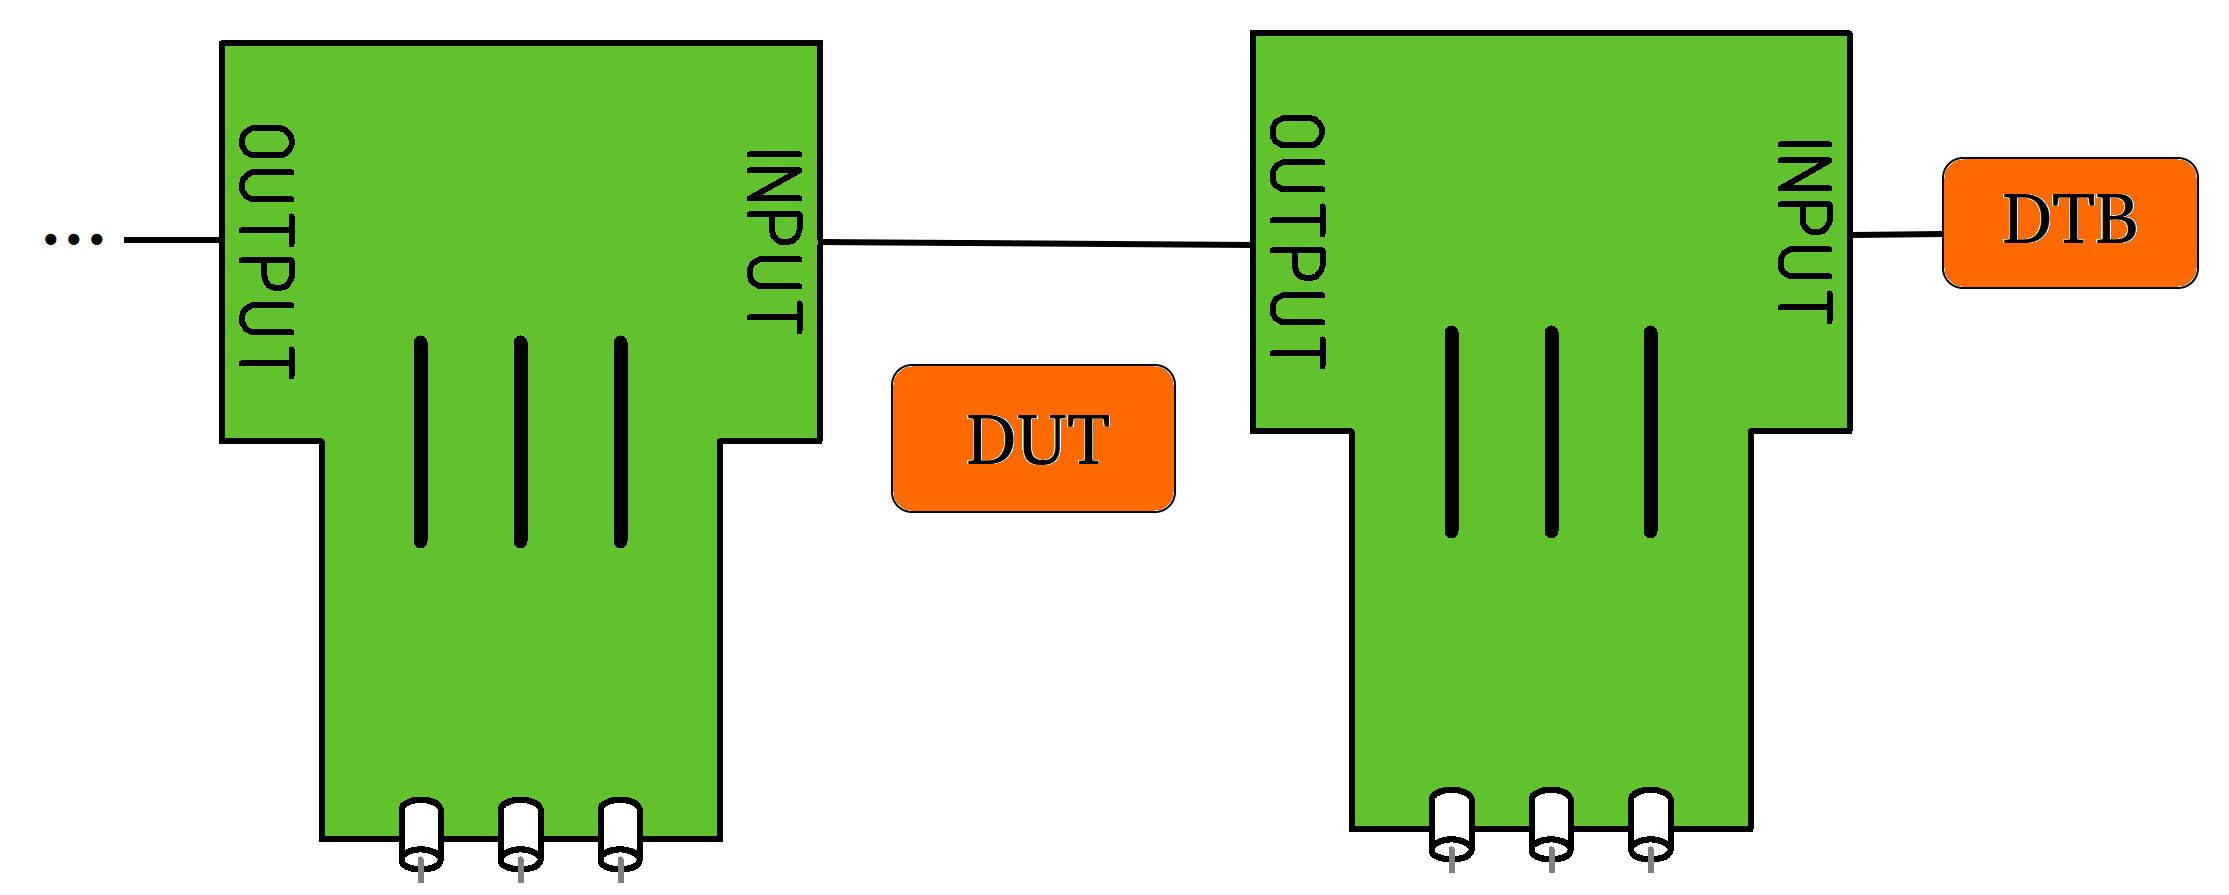
\includegraphics[width=8cm]{Modul}
	\end{center}
	\begin{itemize}
		\item chain several motherboards together into a single big telescope
		\item number of planes per motherboard is also variable 
	\end{itemize}
\end{frame}
% new frame ============================
\begin{frame}
	\frametitle{Diamond Pixel Setup}
	\begin{minipage}{4cm}
		\centering
		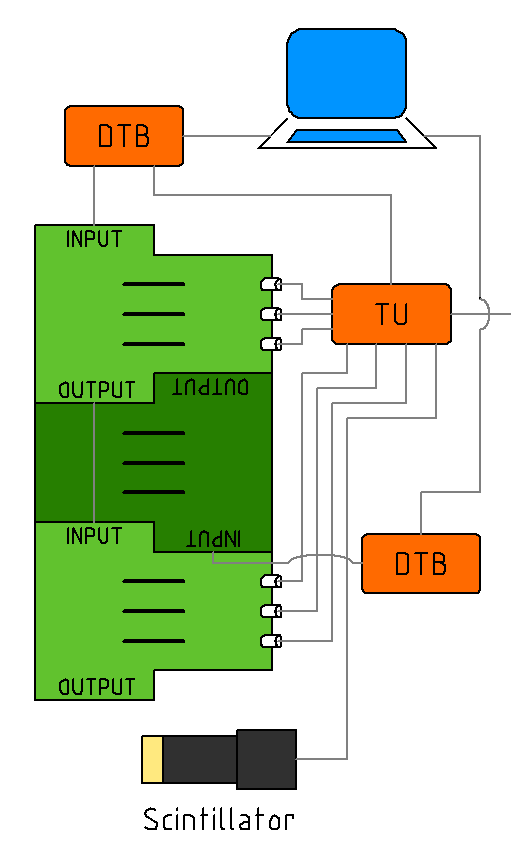
\includegraphics[width=4cm]{fulltel_scint}
	\end{minipage}
	\hspace*{2pt}
	\begin{minipage}{7cm}
		\begin{itemize}
			\item telescope: two motherboards with analogue chips 
			\item DUT: single motherboard with diamonds sensors on digital chips
			\item Scintillator: precise trigger timing 
		\end{itemize}
	\end{minipage}
\end{frame}
% ====================================================================================
% COMMISSIONING
% ====================================================================================
\section{Commissioning}
\begin{frame}
	\begin{alertblock}{
		\begin{center}
			\Large{\textbf{Commissioning}}
		\end{center}}
	\end{alertblock}
\end{frame}
% ============================
% ANALOGUE CHIP
\subsection{Inclusion of the analogue pixel chip}
\begin{frame}
	\frametitle{Inclusion of the analogue pixel chip}
\end{frame}
% new frame ============================
\begin{frame}
	\frametitle{Trigger and clock timing}
\end{frame}
% ============================
% MODULARITY
\subsection{WBC scan}
\begin{frame}
	\frametitle{WBC scan}
\end{frame}
% ====================================================================================
% DATATAKING
% ====================================================================================
\section{Datataking}
\begin{frame}
	\begin{alertblock}{
		\begin{center}
			\Large{\textbf{Datataking}}
		\end{center}}
	\end{alertblock}
\end{frame}
% ============================
% EUDAQ
\subsection{EUDAQ}
\begin{frame}
	\frametitle{EUDAQ}
\end{frame}
% ============================
% PXAR
\subsection{PXAR}
\begin{frame}
	\frametitle{PXAR}
\end{frame}
% ============================
% TRIGGERLOGIC
\subsection{Trigger logic}
\begin{frame}
	\frametitle{Trigger logic}
\end{frame}
% ====================================================================================
% ANALYSIS
% ====================================================================================
\section{Analysis}
\begin{frame}
	\begin{alertblock}{
		\begin{center}
			\Large{\textbf{Analysis}}
		\end{center}}
	\end{alertblock}
\end{frame}
% ============================
% ALIGNMENT
\subsection{Alignment}
\begin{frame}
	\frametitle{Plane alignment}
\end{frame}
% new frame ============================
\begin{frame}
	\frametitle{Event alignment}
\end{frame}
% ============================
% TRACKING
\subsection{Tracking}
\begin{frame}
	\frametitle{Tracking}
\end{frame}
% ============================
% PADS
\subsection{Diamond Pads}
\begin{frame}
	\frametitle{Diamond Pads}
\end{frame}
% ====================================================================================
% CONCLUSION
% ====================================================================================
\section{Conclusion}
\begin{frame}
	\begin{alertblock}{
		\begin{center}
			\Large{\textbf{Conclusion}}
		\end{center}}
	\end{alertblock}
\end{frame}
% new frame ============================
\begin{frame}
	\begin{itemize}
		\item
	\end{itemize}
\end{frame}
% ====================================================================================
% OUTLOOK
% ====================================================================================
\section{Outlook}
\begin{frame}
	\begin{alertblock}{
		\begin{center}
			\Large{\textbf{Outlook}}
		\end{center}}
	\end{alertblock}
\end{frame}
% new frame ============================
\begin{frame}
	\begin{itemize}
		\item
	\end{itemize}
\end{frame}
% ============================
% DOCUMENT END
\end{document}

